\label{ch:cmanager}
%Change this chapter to emulator instead of actual design.
%What am I prototyping here??????????
%Why it is a prototype? Why is it useful? 
%Why an emulator and not an actual system?

In the previous chapters, we discussed the requirements and support of data- and compute-intensive workflows on high performance computing (HPC) resources. 
When considering actual research, scientific projects require to execute multiple workflows at scale and potentially for long period of time.
Usually, workflows are first developed, tested and, when ready, they are executed at scale until the project allocation on the target HPC machine(s) is exhausted. 
This poses unprecedented computing challenges, shifting the problem from enabling the effective and efficient execution of a single workflow at scale, to managing the execution of a computational campaign.

The challenges users face when executing a computational campaign include, but are not limited to, workflow submission, execution and monitoring and deciding an execution plan.
Workflow submission requires from the user to have knowledge of submission systems, which generally are different between HPC resources.
Furthermore, users have to connect to those resources to get information of the execution of a workflow or workflows.
Lastly, users decide an execution plan which defines the order workflows are submitted and executed on HPC resources.
Although, this is feasible for campaigns with small numbers of workflows and resources, it becomes non trivial for campaigns with hundreds of workflows that are executing for months on multiple resources~\cite{smith2020molssi}.
To address these challenges, a campaign manager which given a computational campaign and a set of resources creates an execution plan, submits, executes and monitors workflows on HPC resources, is desirable.

Currently, there are software systems which support computational campaigns, such as PanDA~\cite{maeno2008panda}, DIRAC~\cite{casajus2010dirac}, QCFractal~\cite{qcfractal}, glideinWMS~\cite{sfiligoi2008glidein}, and others.
PanDA WMS~\cite{maeno2008panda}, is built to support the ATLAS experiment~\cite{atlas} at LHC, and is able to execute several thousand jobs concurrently processing million of tasks per week~\cite{de2015future}.
DIRAC~\cite{tsaregorodtsev2003dirac} is LHCb Monte Carlo production system at CERN.
QCFractal~\cite{qcfractal} is a campaign manager to execute upon large scale quantum chemistry data.
GlideInWMS~\cite{sfiligoi2008glidein} is a more general purpose campaign manager as it was designed to support different use cases.
These are domain specific campaign managers and make assumptions about the underlying software stack, and the type of workflows to be executed.

The existing campaign managers also support a plethora of computing resources, including Grid resources, HPCs and Cloud.
PanDA~\cite{maeno2008panda}, glideinWMS~\cite{sfiligoi2008glidein}, and DIRAC~\cite{casajus2010dirac} mainly support grid resources.
PanDA has been extended to support HPC resources~\cite{de2015future, de2016accelerating}, and clouds~\cite{de2016accelerating}, while glideinWMS~\cite{sfiligoi2008glidein} supports clouds.
QCFractal~\cite{qcfractal} supports a set of heterogeneous resources including local campus clusters, HPC resources and clouds.
In addition, there are workflow management systems on HPCs, like Pegasus~\cite{deelman2015pegasus}, and Balsam~\cite{salim2019balsam}, that support the execution of multiple workflows on HPC resources, but not specifically campaigns.

Existing campaign managers are making assumptions about the resources and middleware they are utilizing.
In addition, they are monolithic software systems, despite their modular design, and tend to be domain specific.
For example, PanDA~\cite{maeno2008panda}, Pegasus~\cite{deelman2015pegasus}, and glideinWMS~\cite{sfiligoi2008glidein} are not easily extensible to use other capabilities or runtime systems.
QCFractal is built to be extensible and be able to interface with different workflow and workload management systems. Currently, it supports multiple execution engines.
As a consequence, domain scientists and user either build custom tools to support their needs or fit their campaigns to a selected software system.

In response to these limitations --- monolithic designs, domain specific support and resource and middleware assumptions --- we design and prototype a new campaign manager (CM).
We select to create a prototype instead a production grade system for several reasons.
First, a prototype allows to understand the design space of a campaign manager, its component and basic functionality.
Second, it allows us to quickly implement and test whether the selected design supports the requirements of the use cases.
Third, having a prototype allows us to change the environment of the campaign's execution with minimal cost.

The campaign manager prototype supports use cases from different domains, such as molecular dynamics and earth sciences and as a result, it is domain agnostic.
In addition, our campaign manager is designed by following the building blocks approach~\cite{turilli2019middleware}.
This way, it is agnostic of the system used to manage the execution of the campaign workflows.
In turn, the CM makes no assumptions about the resources on which the campaign workflows will be mapped and executed.

In this chapter, we discuss the campaign manager requirements as they are derived by the use cases it supports.
We describe the building blocks approach, the design architecture and implementation of the campaign manager prototype and how it aligns with the building blocks.
Finally, we characterize the performance  of the prototype.

\section{Campaign manager requirements}
The requirements for designing a campaign manager can be vast.
We use three real use cases to derive the requirements of the campaign manager prototype.
The first use case supports quantum chemistry campaigns, the second earth science and the third data analysis campaigns which analyze the data produced for the ATLAS experiment.

The quantum chemistry use case (UC1) has O(1k) workflows to execute, and up to 1000 to be executing at any given point in time, to a number of different resources. 
The workflows execution time varies between half-core hours up to 100-core hours.
In addition, users have access to resources with several capabilities and not every workflow can be executed in any resources. 

During the campaign definition, the users may provide an initial workflow priority.
This priority may change during runtime, as users want specific workflows to execute before others.
Furthermore, users may want to early bind workflows to resources, as some resources may already support the required software for a workflow, or have the necessary data there.

The set of resources the user has access to and their availability may change during the lifetime of a campaign.
User may get access to new resources as the campaign is executing, and would like to utilize them for the campaign.
In addition, a resource may become permanently unavailable as the user may lose access while the campaign executes.
The campaign may change during runtime as users add or remove workflows.

The earth science use case (UC2) requires the execution of multiple workflows to analyze images from different calendar years.
Workflows are a set of pipelines over an acquired dataset.
Workflow execution time varies from hours to a couple of days.
Workflows are added to the campaign as data are becoming available.
In addition, due to the data volume this use case requires a shared filesystem between the used resources.

A summary of the functional requirements is shown in Table~\ref{tab:fun_reqs}.

\begin{table}[t]
    \centering
    \scriptsize
    \begin{tabular}{@{}p{1.5cm}|p{2.8cm}p{1.5cm}p{6cm}@{}}
        \toprule
        \textbf{REQ ID} &\textbf{Requirement Algorithm} &\textbf{Use Case} & \textbf{Description} \\
        \midrule
         1 & 
         Support campaign with O(1k) workflows & 
         UC1 & 
         The campaign manager should be able to support campaigns with order of thousand workflows.
         Planning, execution and adaptation should be able to execute with such a campaign.\\
         2 & 
         The CM should support at least two different planning algorithms. & 
         G & 
         Users/developers should be able to easily extend the planning capabilities with algorithms.\\
         3 & 
         Support from 1 up to 100 resources & 
         UC1-UC2 & 
         The CM should be able to execute workflows on multiple resources concurrently.
         These resources can either be actual or emulated resources.\\
         4 & 
         Plan should be derived for heterogeneous and homogeneous static resources in 5 minutes & 
         G & 
         The plan should be derived as soon as the user provides a campaign description. 
         Plan should be derived in less than 5 minutes.\\
         5 & 
         Plan should be derived and adapted for heterogeneous/homogeneous dynamic resources in 5 minutes & 
         UC1 & 
         The plan should be derived as soon as the user provides a campaign description.
         Plan should be derived in less than 5 minutes.
         In case the plan needs to be adapted, it should be adapted in less than 5 minutes.\\
         6 & 
         Interface with different WMFs & 
         G & 
         The campaign manager should be able to interface with different WMFs based on the specifics of the campaign. \\
         7 & 
         Early bind workflows to resources &
         UC1 &
         The user may need to bind workflows to specific resources before executing the campaign.\\
         8 & 
         Campaign objective is configurable & 
         UC1 & 
         While the campaign is executing, the objective may be adjusted based on user preferences.\\
         9 &
         Update the campaign during runtime &
         UC1-UC2 &
         The user may want to update the campaign while it is executing to add/remove workflows.\\
         10 &
         Resources may be added or removed during runtime & 
         UC1 & 
         The user may want to add/remove resources, she has gained/lost access to.\\
        \bottomrule
    \end{tabular}
    \caption{Campaign manager functional requirements.\label{tab:fun_reqs}}
\end{table}

\section{Campaign Manager Design}
This section discusses the design principles and the architecture of the campaign manager prototype.
The design principles the campaign manager follows are presented in ~\S~\ref{ssec:building_blocks}.
The architecture and API of the campaign manager is described in \S~\ref{ssec:cm_arch}.
\subsection{Building Blocks Design Approach}
\label{ssec:building_blocks}
The building blocks approach, as descirbed in~\cite{turilli2019middleware}, defines four design principles for software systems.
Those are self-sufficiency, interoperability, composability, and extensibility.
Adhering to those principles during the design and implementation phase of a software system allows for greater software sustainability.
In addition, it allows users to not tailor their solutions to a specific software ecosystem and take full advantage of the plethora of software that supports scientific computing.

Self-sufficiency and interoperability describe the characteristics of software entities and functionalities.
The entities are enough to stand alone and can be reduced to a specific abstraction.
The functionalities of each building block are specific to the block and do not overlap with other blocks.
As a result, the campaign manager design defines a set of components and that allow it to execute a campaign to HPC resources without providing capabilities to execute the individual workflows of the campaign or acquire the necessary resources.

Composability and extensibility describe the communication and coordination between building blocks and the generality of the generality of the blocks components respectively.
Blocks communicate information about their state, events and errors.
Based on this information alone building blocks are coordinating with each other.
As a result, the campaign manager uses only the state of the workflow execution to create the campaign state.
Furthermore, its components are designed to be general enough so that they can extended and interface with different workflow execution engines as well as software systems that execute computational campaigns.

\subsection{Campaign Manager Components}
\label{ssec:cm_arch}

Figure~\ref{fig:refarch} shows a reference architecture where the CM has three components:
\begin{inparaenum}[(1)]
    \item a Planner;
    \item an Enactor; and
    \item a Bookkeeper. 
\end{inparaenum}
Workflow execution will be managed by an existing workflow management framework (WMF) on HPC resources.
Plan updates will be based on workflows execution metrics provided by the selected WMF such as tasks execution time, overheads calculation and time to completion.
These metrics will be aggregated across workflows, resulting in campaign-wide execution metrics.

\begin{figure*}[t]
    \centering
    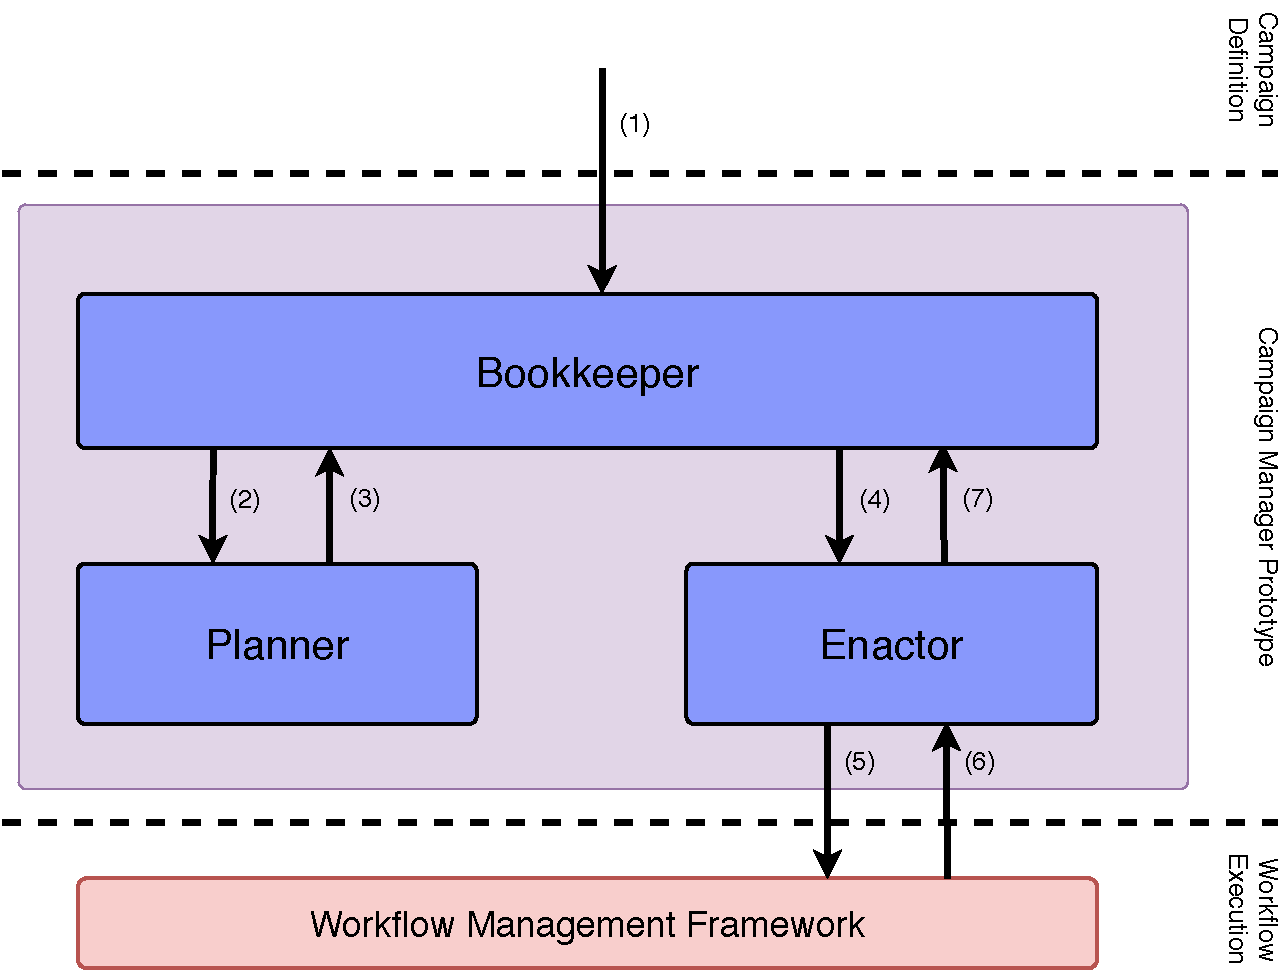
\includegraphics[width=.95\textwidth]{figures/manager/CEM_design.pdf}
    \caption{Reference Architecture of a Campaign Manager. Basic 
        components of Campaign Manager (CM): 1) Planner, 2) Enactor and 3) Bookkeeper. 
        CM communicates decisions to Workflows Management Framework. CM communicates with HPCs to 
        execute parts of the campaign.}\label{fig:refarch}
\end{figure*}

The planner derives an execution plan based on a planning algorithm, calculates the makespan of a campaign based on the set of available resources and the given objective. 
The planner receives information about the state of resources as well as the state of the workflows of the campaign from the bookkeeper component.
In addition, based on information from the other components, the planner might be able to update the plan during the campaign runtime. 

The Bookkeeper component is responsible for monitoring the execution of the campaign.
This component knows the state of the campaign, the execution plan, the availability of the resources, and the campaign's objective.
The state of the campaign will be based on information that the bookkeeper receives from the enactor component.
In addition, the bookkeeper knows the state of the resources the campaign is utilizing at runtime and the state of the resources that are planned to be used.
Based on this set of information, the bookkeeper checks whether the campaign's objective can be achieved.
The bookkeeper will inform the planner to update the plan when changes in the campaign happens that affect the effectiveness of a current plan or make the stated objective not achievable. 
For example, workflows could be removed or added to the campaign, or the availability of one or more resources could change requiring a revision of the mapping of workflows to resources or making such mapping impossible.

The enactor is responsible to execute the planner's plan by interfacing with the WMF.
Based on the plan, the enactor is responsible to execute workflows on the assigned resources.
To achieve that, the enactor informs the WMF to acquire resources, translates the workflow from the user's specification to the API provided by the WMF, and submits the workflow for execution.
Furthermore, the enactor informs the bookkeeper about which workflows were submitted for execution and their state.
%In the case where a group of workflows is to be executed as a single workflow, the enactor will be responsible to group them as well.

\section{Prototype Implementation and Performance Evaluation}
\label{sec:cm_impl}

The campaign manager prototype in accordance with its design defines three major classes.
A bookkeeper class implements the capabilities of the bookkeeper component.
An enactor class interacts with a selected workflow engine to execute worklflows on resources.
A planner class that implements planning algorithms.
In addition, it defines a state model for the campaign and the workflows.

The states models provide information about the state of the execution.
The campaign state model has four states: 1) \textit{new}, 2) \textit{planning}, 3) \textit{executing}, 4) \textit{done}, 5) \textit{canceled} and 6) \textit{failed}.
A campaign is considered \textit{new} when it is defined and no further action is taken.
It goes to state \textit{planning} when a plan for its execution is derived.
As soon as the execution of the campaign starts, the state transitions to \textit{executing}.
The final state is a set of possible termination states.
When the campaign execution ends and the campaign objective is achieved, the state transitions to \textit{done}.
If the objective cannot be achieved or there is a failure during the execution, the state changes to \textit{failed}.
Lastly, the campaign state goes to \textit{canceled} when the user cancels the execution of the campaign.

The workflows state model defines three states: 1) \textit{new}, 2) \textit{executing}, 3) \textit{done}, 5) \textit{canceled} and 6) \textit{failed}.
A workflow is in \textit{new} state when it is received by the bookkeeper.
Its state transitions to \textit{executing} when the enactor submits the workflow for execution to the selected workflow management system.
A workflow state transitions to one of the final states based on the final state the workflow management system reports.

Figure~\ref{fig:rcm_class_diagram} shows the class diagram of the prototype.
We define three classes based on each component of the reference architecture.
Each class also defines a set of data structures to support the execution.

\begin{figure*}[t]
    \centering
    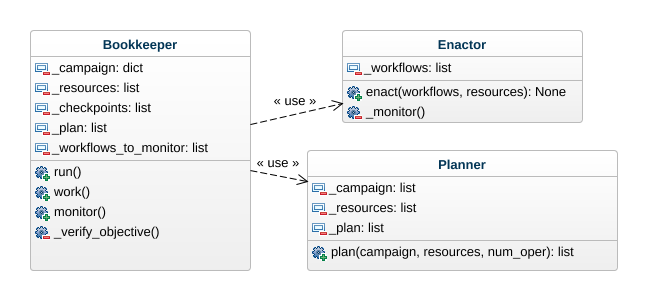
\includegraphics[width=.95\textwidth]{figures/manager/class_diagram.png}
    \caption{Class diagram of campaign manager prototype}\label{fig:rcm_class_diagram}
\end{figure*}

The Bookkeeper class defines the necessary methods to execute a campaign.
The most important methods are \textit{run}, \textit{work} and \textit{monitor}.
Method \textit{run} initializes the campaign state to \textit{new} and sets up the environment for executing the campaign.
\textit{Work} calls the planner to produce a plan transitioning the state of the campaign to \textit{planning}.
After a plan is produced, \textit{work} via calling \textit{\_verify\_objective} checks if the objective of the campaign can be achieved and starts submitting workflows to the enactor.
In addition, it pushes the submitted workflows to a data structure that the \textit{monitor} method reads.
The \textit{monitor} method checks the state of the workflow execution as given by the enactor.

The planner and enactor classes define the methods for planning the execution of a campaign, executing workflows on resource and monitoring their execution.
The planner defines a \textit{plan} method which implements a planning algorithm.
The \textit{enact} method submits a workflow to a resource for execution by calling the selected workflow management framework.
The \textit{monitor} method checks periodically the state of the workflows that are executing and updates it accordingly.

\begin{figure*}[t]
    \centering
    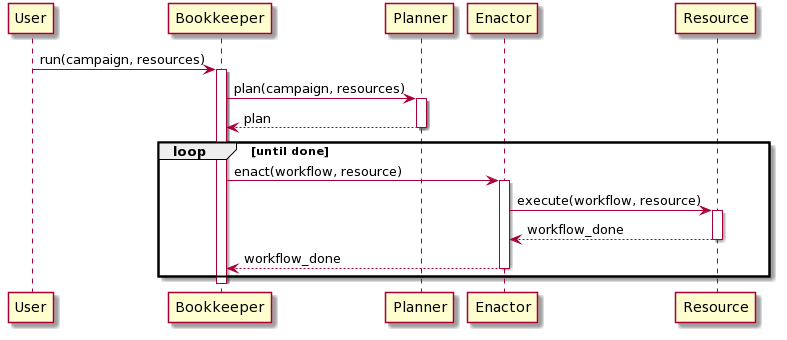
\includegraphics[width=.95\textwidth]{figures/manager/rcm_seq.png}
    \caption{Sequence diagram for executing a computational campaign through the campaign manager prototype}
    \label{fig:seq_diag}
\end{figure*}

During the execution of a campaign there is a specific sequence of actions that happen.
FIgure~\ref{fig:seq_diag} shows the sequence diagram of the execution.
Before the execution of a campaign the bookkeeper gets as input a campaign ( a set of workflows) and a set of resources.
As the user requests from the prototype to execute the campaign, the bookkeeper passes to the planner the information it needs.
As soon as the plan is ready, the execution of the campaign begins with the bookkeeper passing a workflow along with the resource that it will run to the enactor.
As the enactor executes the workflow, it pushes state updates to the bookkeeper via callbacks, updating the state of the workflows for the bookkeeper.
The bookkeeper continues to pass workflows to the enactor as resources become available and as long as there are workflows that are not executed.

The execution of a campaign can span from months to a year and any experimentation with a prototype is almost unfeasible.
For this reason, we utilize a discrete time simulator, SimPy~\cite{simpy}.
The simulator advances time which, in turn, allows the CM's components to recognize the state of the execution and take the necessary actions.
As a result, we are able to test and identify possible bottlenecks in the design or our implementation.

\begin{figure*}[ht!]
    \centering
    \begin{subfigure}[b]{0.75\textwidth}
        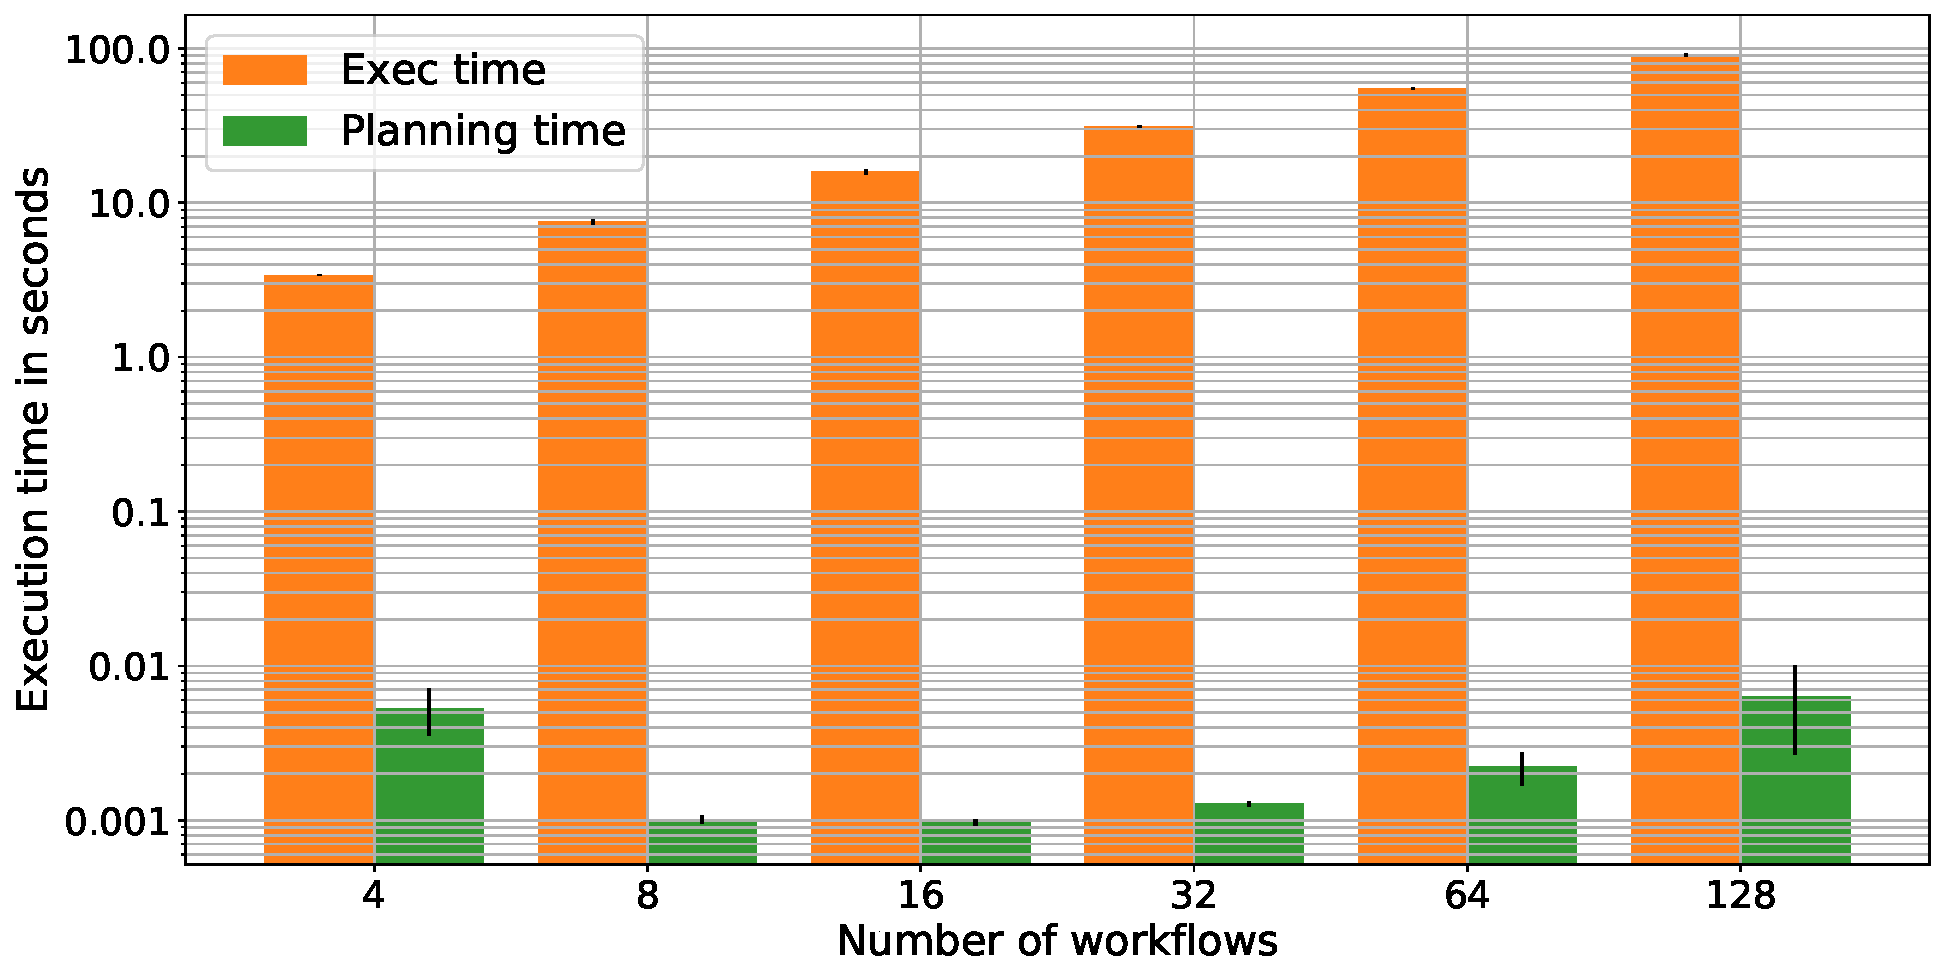
\includegraphics[width=.95\textwidth]{figures/manager/SimTimeWork.pdf}
        \caption{}
        \label{fig:SimTimeWork}
    \end{subfigure}\\
    ~ 
    \begin{subfigure}[b]{0.75\textwidth}
        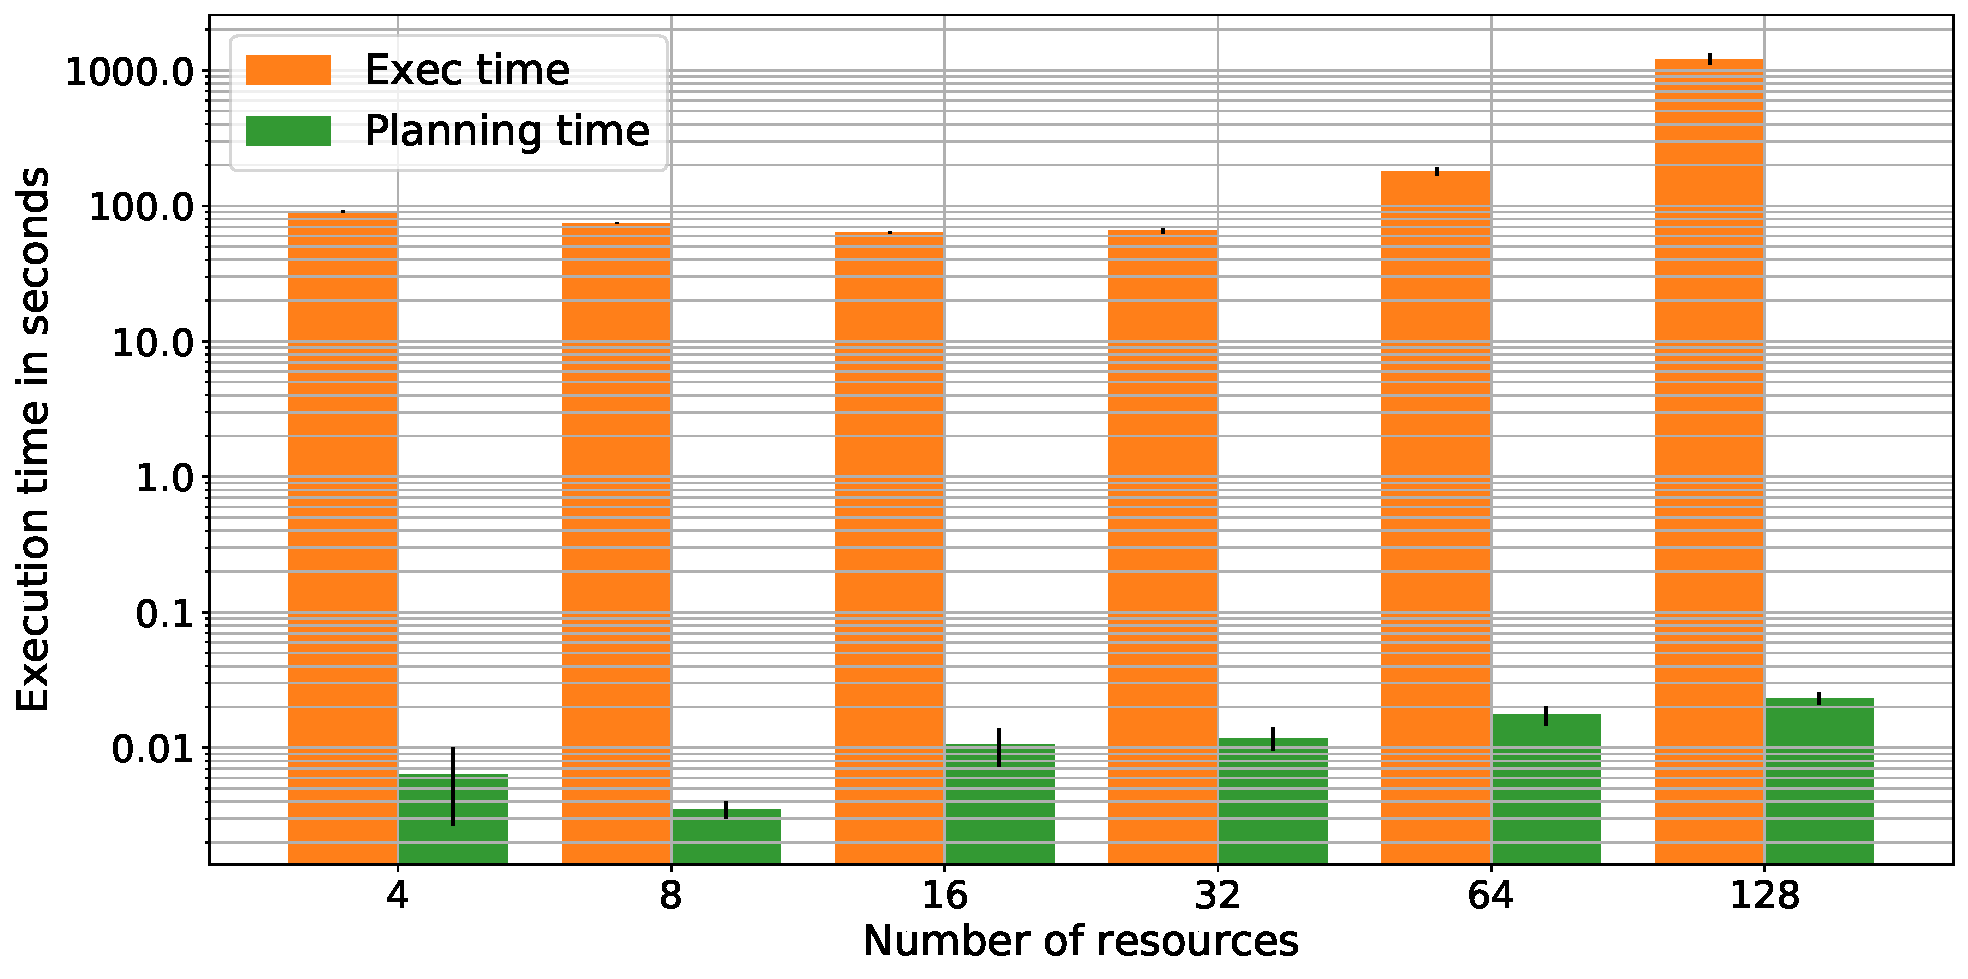
\includegraphics[width=.95\textwidth]{figures/manager/SimTimeRes.pdf}
        \caption{}
        \label{fig:SimTimeRes}
    \end{subfigure}
    \caption{Execution time of simulating the execution of a computational campaign with: ~\ref{fig:SimTimeWork}) different number of workflows on 4 resources;~\ref{fig:SimTimeRes}) campaign with 128 workflows and different number of resources.}
    \label{fig:cm_char}
\end{figure*}

Figure~\ref{fig:cm_char} shows the performance characterization of the prototype with the simulator.
We measured the time it takes the prototype to execute campaigns of different size while we kept the number of resources constant and a campaign with constant number of workflows executing on different number of resources.
The bookkeeper submits workflows for execution until all workflows have finished.
As a result, the time the simulator runs is linear to the number of workflows.
Figure~\ref{fig:SimTimeWork} shows the time it takes the simulator to execute 4 to 128 workflows on 4 resources and verifies the expectation that the execution time of the simulation is linear.
On the other hand, the number of resources should not affect the execution time of the simulation.
This is generally true up to 32 resources, as we see in figure~\ref{fig:SimTimeRes}.
Above 64 resource, the time of the simulation doubles.
The enactor monitors all workflows that are executing via traversing a list and uses a callback for those that finished.
In addition, the bookkeeper checks the state of the workflows that are executing.
Increasing the number of resources means that the number of workflows increases and above 64 resources these two checks start to dominate the execution time.


\section{Conclusions}

In this chapter, we motivated and discussed a prototype for a software system that supports the execution of computational campaigns on HPC resources based on a set of use cases.
We described the design and the basic components of the campaign manager, a bookkeeper, a planner and an enactor.
Based on the selected design, we implemented a software prototype that simulates the execution of a campaign on resources.
The prototype allows us to understand and correctly implement the necessary functionality of the campaign manager.

We used the prototype to simulate the execution of campaigns with different number of workflows and different number of resources.
Based on our execution results, we see that we are able to simulate a campaign of 128 workflows to 128 resources in around 15 minutes.
In addition, we saw that the execution times are linearly proportional to the number of workflows.
Further, we saw that the number of resources can affect the execution time of the simulation when the number of resources is more than 64.
The analysis of this unexpected behavior provides us with an idea which parts of the campaign manager may show significant overheads when it is used in production.

